
\subsection{AWS Amplify}

Amplify ist ein zentraler Dienst rund um das Thema Serverless Webanwendungen, die Veröffentlichung war im November 2017.

Amazon bezeichnet Amplify selbst als {}\glqq ein Set aus Tools und Services, das Entwicklern erlaubt, skalierbare vollständige
mobile und Front-End-Anwendungen zu entwickeln, powered by AWS.\grqq{}\cite[]{AWSAmplify}

Amplify lässt sich sowohl über die Amazon Web Console konfigurieren, als auch über eine eigene Amplify CLI.
Das Amplify Framework ist Open Source und vereint native AWS Dienste zur Authentifizierung, Analyse, CI/CD, Hosting, Datenspeicherung für Desktop und Mobile
Endgeräte. Dabei werden viele moderne Javascript Frameworks zum Aufbau des Frontends unterstützt, wie zum Beispiel React, React Native, Vue und weitere.
Alle verfügbaren Dienste sind in der Amplify Bibliothek vereint und können in das Frontend eingebaut werden.

Amplify erleichtert es einem Projekte als Full Stack Developer\footnote{Als Full Stack Developer wird jemand bezeichnet, der sowohl Client als auch Server
erstellen und betreuen kann. Er ist allein Verantwortlich für das Frontend, Backend und eventuell damit verbundene Datenbanken.} zu realisieren.
Dies ermöglicht einem ein voll umfängliches Verständis über die gesamte Applikation und Änderungen können leichter durchgeführt werden.
Ein Prototyp kann ebenfalls schnell erstellt werden.

Das Amplify Framework lässt sich in drei Komponenten unterteilen: Bibliotheken, UI-Komponenten und einer CLI Toolchain, wobei jede Komponente einzeln oder gemeinsam genutzt werden kann.

Die Bibliotheken sind Open Source und nutzen bereits vorhandene AWS Dienste um eine native Webanwendung für die Cloud bereitzustellen.
Folgende Module stehen zur Verfügung:

- Voll verwaltete Authentifizierung mit Unterstützung für Social Media Logins, wie Facebook, Google Sign-In. Multifaktorauthentifizerung, Authorisierung und Passwortwiederherstellung sind
bereits inkludiert. Zugrundeliegender Dienst ist Amazon Cognito.

- DataStore zur Offline-Synchronisation zwischen mehreren Plattformen. (iOS/Android/React Native/ Webbrowser). Zugrundeliegender Dienst ist AWS AppSync.

- Echtzeitanylsen erstellen und auswerten sowie integriertes Tracking von Sessions. Zugrundeliegender Dienst Amazon Pinpoint und Amazon Kinesis.

- API Zugriffe auf Endpunkte mithilfe von GraphQL oder REST erstellen, sowie manipulieren und kombinieren von Daten unterschiedlicher Quellen. Zugrundeliegender Dienst ist Amazon AppSync und Amazon API Gateway.

- Simple Speicherverwaltung in öffentlichen oder privaten Storage Buckets. Kann auch benutzt werden um Useruploads zu verwalten. Zugrundeliegender Dienst ist Amazon S3.

- Zudem gibt es noch weitere Funktionen, wie Publish/Subcribe, Chatbots, Push Benachrichtungen, AR/VR sowie Künstliche Intelligenz.
--> Erklärung der einzelnen Dienste mit Fußnote??


Auch die UI-Komponenten sind Open Source und sollen eine einfache Verzahnung zwischen dem User Interface und den Workflows der Dienste anbieten.
So gibt es zum Beispiel fertige Interace Elemente für das Hochladen von Bildern und Datein in S3.

Die Amplify CLI Toolchain dient dazu, ein Serverless Backend zu erstellen und verwalten. Dazu gehört die Erstellung aller zuvor genannten Dienste und Funktionen. Zudem
ist es möglich ein Statisches Hosting einzurichten. \cite[]{AWSAmplifyKomponenten}


Um alle unterschiedlichen AWS Dienste verwalten zu können nutzt Amplify einen weiteren AWS Dienst, AWS CloudFormation.
Mit AWS CloudFormation ist möglich Templates zur Modellierung und Bereitstellung jedlicher AWS Ressourcen zu erstellen. Die Templates unterstützen
JSON und YAML. Amplify übersetzt alle Befehle in ein Cloudformation Template und startet dieses. Dadurch ist es einfach alle, von Amplify durchgeführten Schritte,
nachzuvollziehen und eventuell für andere Projekte zu übernehmen.

Im folgenden Schritt werden die einzelnen Dienste erläutert die für diese Bachelorarbeit und Implementierung notwendig sind.
Zudem folgt eine Bewertung zur Eignung des jeweiligen Dienstes.




\subsection{API}
API steht für Application Programming Interface und bezeichnet eine Programmierschnittstelle für die Kommunikation von Diensten.
Zur einfacheren Handhabung und höherer Flexibilität sollen Daten über einen standardisierten Weg ausgetauscht werden. Die API definiert
dabei die Art und Weise der Kommunikation, also wie Daten angenommen, verarbeitet und wieder zurückgesendet werden.


Amazon bietet zwei Möglichkeiten an eine solche API zu erstellen welche im folgenden Schritt gegenüber gestellt werden.
Einer der beiden Dienste wird anschließend für die Implementierung der Anwendung genutzt.


\subsubsection{REST API: AWS API Gateway}
Das Grundprinzip der REST (REpresentational State Transfer) API Architektur ist es eine strukturierte Kombination aus Ressourcen und Methoden zu erhalten.
Ressourcen bestehen aus sogenannten URI (Unified Resource Identifier), und geben Inhalte in JSON oder XML zurück.
Mittels den zustandslosen HTTP-Methoden GET, POST, PUT und DELETE kann mit Servern im Internet agiert werden.
Laut Anforderungen soll sich REST an das Client-Server Modell halten und unabhängig voneinander funktionieren können.
Der Client hat jederzeit die Möglichkeit Daten vom Server anzufordern.
Die gewünschten Daten sind immer über eine spezifische URI identifizierbar.

Beispiel für Abfragen könnten folgendermaßen aussehen:
\begin{lstlisting}
 GET /AccountNames/
 GET /AccountNames/123
 GET /AccountEmail/12
 POST /Accounts/1
\end{lstlisting}

Mithilfe des ersten GET Requests kann eine Liste von Accounts abgerufen werden, der zweite GET Request liefert nur die Informationen für den 123 Eintrag der Accountnamen.
Um nur zwei Namen zu erhalten sind dementsprechend auch zwei Requests notwendig, da sie separate Ressourcen sind.
Die andere Option ist es alle Accountnamen zu erhalten und nur die benötigten heraus zu filtern.
Der POST Request erlaubt es einen neuen Account anzulegen.
Es ist wichtig vorher zu überlegen in welchem Kontext die Daten später benötigt werden.

Dank der Zustandslosigkeit wird eine leichtere Skalierung ermöglicht. Anfragen können durch einen Loadbalancer auf mehrere Server verteilt und bearbeitet werden.
Auch ist eine Cache Implementierung mithilfe von REST leicht
umsetzbar. Wächst eine Applikation immer weiter entstehen auch immer neue API Endpunkte. Möchte man nun alle Daten sammeln wären mehrere separate
Anfragen notwendig. Es ist zudem nicht möglich die angeforderten Daten genauer zu spezifizieren. Mittels GET Request erhält man immer alle Daten die
die API zurückgibt, egal wie viel man tatsächlich davon benötigt. Dieses Phänomen nennt sich Over-fetching bzw. Under-fetching.
Beim Over-fetching werden mehr Daten bezogen als die Anwendung eigentlich benötigt und beim Under-fetching müssen mehrere Anfragen an den Server
gesendet werden um die benötigte Menge an Daten zu erhalten.\cite[]{API}


AWS API Gateway ist ein vollständig verwalteter Service um solche API Endpunkte zu erzeugen.
Dabei steht er als zentrale Schnittstelle zwischen Endgeräten und Backend-Diensten. Zu den Endgeräten zählen Webanwendungen, Mobilgeräte oder auch
IoT\footnote{IoT steht für Internet of Things (deutsch: Internet der Dinge) und bezeichnet ein System von vernetzten Geräten, welche
 über das Internet miteinander kommunizieren können. Dazu gehören Geräte die ihre Daten selbständig sammeln und zur Verfügung stellen können,
 etwa auch Alltagsgegenstände wie smarte Thermostate oder digitale Sprachassistenten. } Geräte.
Anfragen werden vom Gateway anschließend je nach Konfiguration verarbeitet.
Mithilfe des Dienstes lässt sich beispielhaft die zuvor beschriebene GET Anfrage an eine Datenbank weiterleiten, die die gewünschten Daten zurückgibt.
Die POST Anfrage könnte eine Lambda-Funktion verarbeiten, welche wiederum die neu erhaltenen Daten in die Datenbank speichert.
AWS API Gateway arbeitet dabei vollkommen Serverless und skaliert automatisch mit den Anforderungen. Neben Zugriff auf den Lambda Dienst, ist es auch möglich
mit anderen Diensten wie EC2, S3 oder auch DynamoDB zu kommunizieren.

Zusätzlich bietet der Dienst viele weitere Funktionalitäten. Dazu gehören CORS-Support\footnote{CORS steht für Cross-Origin Resource Sharing und
beschreibt einen Mechanismus der mittels zusätzlicher HTTP Header Berechtigungen für Ressourcen vergibt, falls sich diese Ressourcen auf einer anderen
Domain befinden als auf der eigenen.}, eine Zugriffskontrolle und Einschränkung, oder auch die Verwaltung unterschiedlicher
API-Versionen. Es ist auch möglich mit OnPremises Servern zu kommunizieren und Anfragen weiterzuleiten.\cite[]{APIGateway}

Die Abrechnung erfolgt anhand von API-Aufrufen und Datenübertragungen die in Richtung Internet verlaufen. Eine Pauschale gibt es nicht.
Für die ersten 333 Millionen Anfragen pro Monat kosten in der Region Frankfurt eine Millionen API-Aufrufe 3,70 USD. Hat man mehr als 333 Millionen
Aufrufe sinkt der Preis weiter. Bei über 20 Milliarden Aufrufen kosten 1 Millionen API-Aufrufe nur noch 1,72 USD.
Darüber hinaus entstehen kosten falls man Caching nutzen möchte, und eine bessere Leistung für seine API benötigt. Hier kosten 0,5 GB an Zwischenspeicher
0,02 USD pro Stunde. Je höher der Speicher, desto höher auch der Stundensatz.
\cite[]{APIGWPrice}

\subsubsection{GraphQL API: AWS Appsync}

2015 wurde GraphQL von Facebook veröffentlicht und 2018 in die Linux Foundation\footnote{Die Linux Foundation ist eine Gemeinnützige Organisation mit Sitz in der USA.
Das Ziel ist es Linux zu fördern und den Wachstum zu unterstützen.} ausgegliedert.
GraphQL APIs arbeiten nicht mit Ressourcen oder HTTP Methoden.
Stattdessen ist es wichtig zu Beginn ein statisches Schema mit der GraphQL Schema Definition Language zu erstellen
Das Schema legt die Regeln fest wie der Client auf Daten zugreifen kann.
Datentypen müssen im vorraus definiert sein.
Zudem muss festgelegt werden, ob es sich um eine Mutation oder eine Query handelt.

Eine Query ist eine einfache Abfrage der Daten, eine Mutation ermöglicht eine Veränderung der Daten.
GraphQL erlaubt, anders als REST, nur bestimmte Daten in einer Abfrage abzurufen. Ein Over- bzw. Under-fetching gibt es hier nicht.
Im Vergleich zu REST ist GraphQL flexibler und benötigt weniger Änderungen im Backend. Der Client hat mehr Möglichkeiten
mit der API zu kommunizieren, da er selbst entscheiden kann wie er Daten abfragt. Ein Vorteil der stark definierten Typen ist
eine geringere Fehlkommunikation zwischen Server und Client.
Der Server kann die Anfragen automatisch auf Korrektheit prüfen und fehlerhafte Anfragen bereits zu Beginn der Transaktion ablehnen.

Ein Schema würde man mit GraphQL wie folgt darstellen:
\begin{lstlisting}
type Account {
  id: ID!
  accountid: String!
  name: String!
  email: String!
  num: Int!
  status: String!
}
\end{lstlisting}

Den einzelnen Felder wird zugewiesen ob es sich um ein String, Int oder etwas anderes handelt. Mit dem Ausrufezeichen wird ein Feld als zwingend benötigt markiert.
Es darf also nicht leer sein. Die einzigartige ID wird vom Server beim erzeugen von neuen Einträgen automatisch erstellt.

In GraphQL würde eine Query folgendermaßen aussehen:
\begin{lstlisting}
query listAllAccounts {
  listAccounts {
      id
      accountid
      num
      name
      email
  }
}
\end{lstlisting}

Die Query gibt alle aufgelisteten Daten zurück.
Wird zum Beispiel die Email nicht benötigt, lässt man das Feld weg und die Information wird nicht mehr an den Client übertragen.
Zum Hinzufügen eines neuen Eintrags wäre folgende Mutation notwendig:
\begin{lstlisting}
mutation {
  createAccount(
      name: "AWS-XXX",
      num: 145,
      email: "oktavius@cbc.de",
      accountid: "123456789",
      status: "ACTIVE)
       {
        id
      }
}
\end{lstlisting}

Es ist außerdem möglich in einer Mutation auch direkt Daten abzufragen. Beim Erstellen eines neuen Accounts kann man gleichzeitig die
vom Server angelegte ID abfragen und überprüfen.


Neben den bisher genannten Funktion bietet GraphQL noch Subscriptions an.
Diese ermöglichen dem Client Echtzeitbenachrichtigungen zu erhalten, sobald neue Daten dem Backend hinzugefügt worden sind.
Dadurch dass GraphQL, anders als REST, nur einen einzelnen Endpunkt anbietet, ist eine Cache Implementierung problematischer.
Bei einer REST API ist es möglich für jeden GET Request ein Cache-Control Header in der HTTP Anfrage zu implementieren, wodurch der Client das Caching übernehmen kann.
Bei GraphQL muss zusätzlicher Code im Client implementiert werden oder das Schema entsprechend angepasst werden. Der Dienst Apollo Server ermöglicht es
eine GraphQL API bereitzustellen, die bereits Cache Header unterstützt. Dafür muss die Option \glqq{}cacheControl\grqq{} in das Schema eingebaut werden. Es ist auch möglich
die Option für jedes individuelle Feld zu setzen. \cite[]{Apollo}
Dadurch dass die Definition des Schemas mehr Zeit in Anspruch nimmt dauert es im Vergleich zu REST länger bis man erste Abfragen durchführen kann. \cite[]{GraphQL} \cite[]{GraphQL1}

Damit GraphQL weiß welche Operationen es bei Anfragen durchführen soll werden Resolver benötigt.
Resolver sind Funktionen welche bestimmen wie jedes einzelne Feld im Schema weiterverarbeitet wird.
Es ist nicht möglich Resolver direkt im Schema anzugeben, sie müssen außerhalb erstellt werden. Im Resolver kann auch
angegeben werden, dass eine Funktion aufgerufen werden soll.

\clearpage
Mithilfe von AWS Appsync ist es möglich APIs bereitzustellen die auf GraphQL basieren. Dabei ist AppSync in viele weitere AWS Dienste integriert.
Das folgende Schaubild von Amazon zeigt die Funktionsweise des Dienstes genauer.
\begin{figure}[htbp]
    \centering
    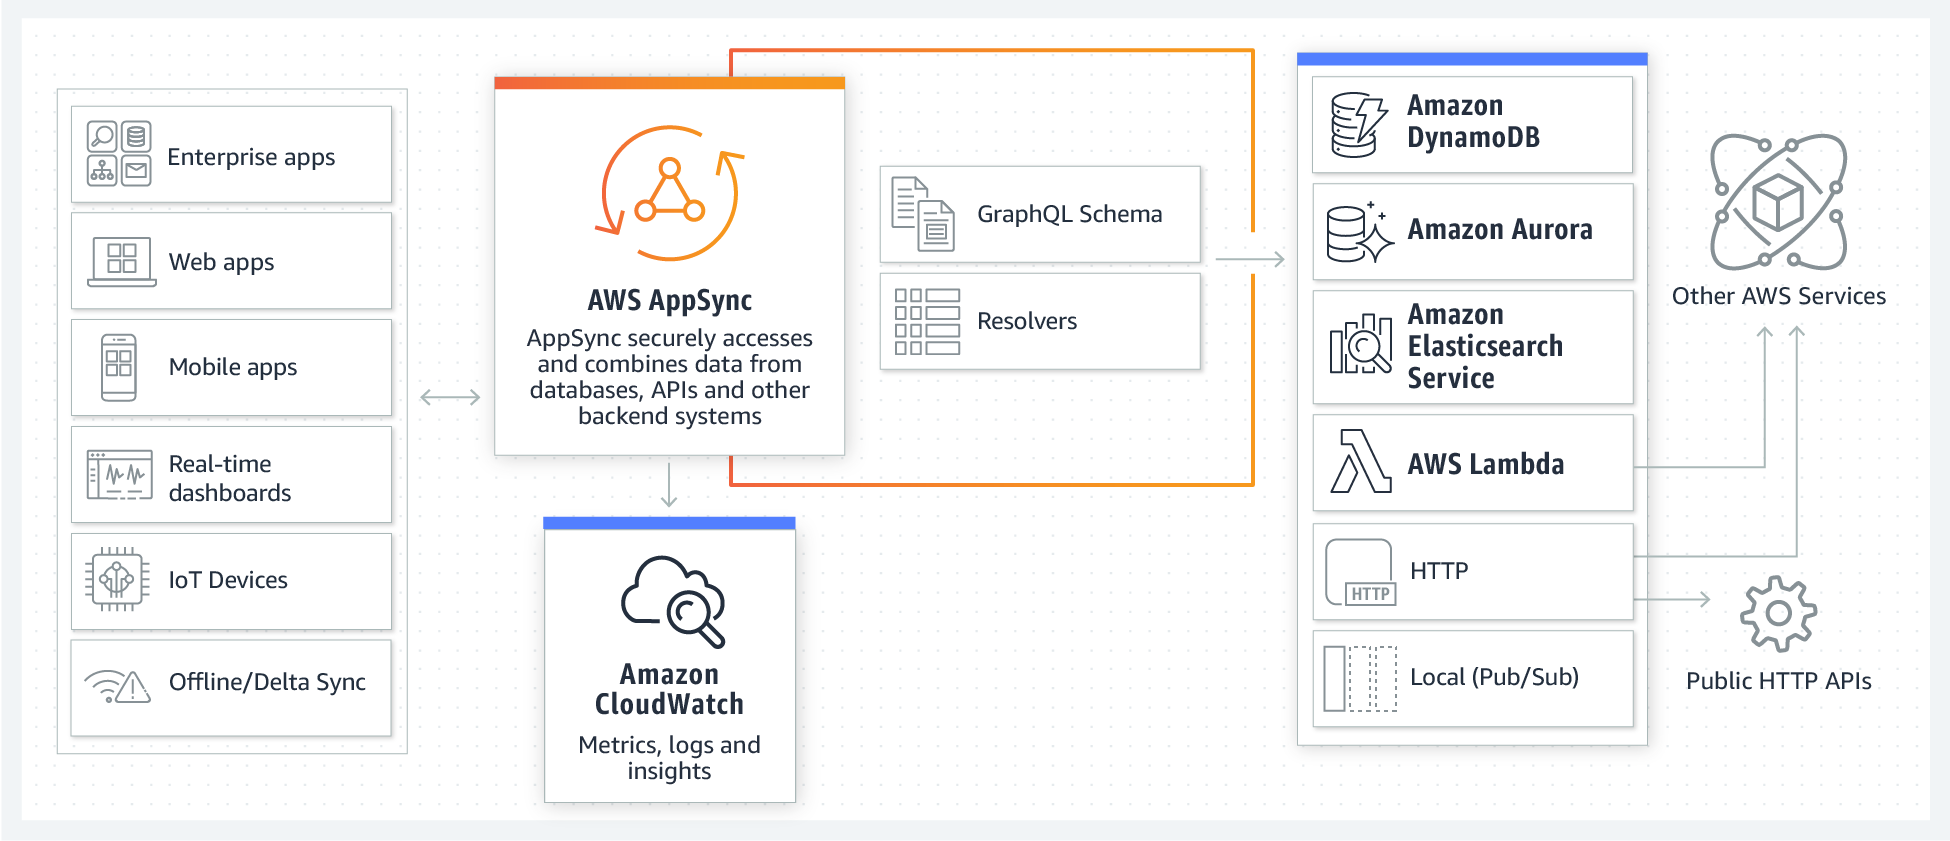
\includegraphics[width=1.0\textwidth]{40-AWS/Appsync.png}
    \caption{Funktionsweise von AppSync \cite[]{AppSync}  }
    \label{fig:meine-grafik}
\end{figure}

So kann man direkt über AppSync eine NoSQL Datenbank mit AWS DynamoDB (Siehe XXX) und allen benötigten Berechtigungen aufsetzen.
AWS stellt zudem auch alle benötigten Resolver für die Kommunikation zur Verfügung und kann auch auf Wunsch ein Schema erstellen. Durch die Resolver wird die Datenbank mit
der API verknüpft und alle möglichen Queries und Mutationen erstellt. Darüber hinaus ist es möglich auch eigene Resolver zu erstellen, falls dies benötigt wird.
Auch mit AWS Lambda und AWS Cognito( siehe XXX) ist der Dienst verbunden.
Die Autorisierung von Clients ist mit API Keys\footnote{Der API Key wird nur für Entwicklungsumgebungen empfohlen,
da er leicht kompromittierbar ist und keine Aufteilung von Berechtigungen ermöglicht.}
, IAM Credentials \footnote{
    IAM steht für Identity Access Management und beschreibt Amazons Dienst zur Identität- und Benutzerverwaltung. Der Dienst erlaubt es Nutzer anzulegen und
    Ihnen Berechtigungen zu verteilen.}, OIDC Tokens \footnote{OIDC steht für OpenID Connect und basiert auf dem OAuth 2.0 Protokoll zur Authentifizierung.
    Die Tokens zur Authentifizierung (JWT Tokens) einer Identität werden verschlüsselt im JSON Format versendet, und ermöglichen einen standardisierten Weg zum Anmelden.
          } oder einem AWS
Cognito User Pool ( siehe XXX) möglich. \cite[]{AppSyncAuth}

Das AppSync SDK unterstützt iOS, Android und viele Javascript Varianten wie React, React Native oder Angular und kann mit dem Apollo Client genutzt werden.
Auch Echtzeitanwendungen können mit AppSync und GraphQL Subscriptions realisiert werden.
Zusätzlich bietet Amazon ein serverseitiges Caching von Daten an, um direkten Zugriff zu reduzieren und die Geschwindigkeit zu erhöhen. Für das Caching wird
der AWS Dienst ElastiCache verwendet, der auf den Memory-Speicher Redis basiert.
Um Caching nutzen zu können, ist es notwendig einen Instanztypen mit bestimmter Kapazität auszuwählen. Der kleinste auswählbare Instanztyp \glqq cache.small\grqq{}
mit einer vCPU und 1,55 GB Arbeitsspeicher kostet zum Beispiel 0,044 USD pro Stunde.
Eine Millionen API-Aufrufe kosten 4,00 USD, eine Vergünstigung bei mehr Abrufen gibt es im Vergleich zu API Gateway nicht.
\cite[]{AppSync} \cite[]{AppSyncPreise}



\subsubsection{Entscheidung}
Für das, in dieser Arbeit, gewünschte Projekt wäre eine Implementierung sowohl mit einer REST API als auch mit GraphQL möglich.
Beide Dienste für die API sind zudem direkt in Amplify integriert und benötigen keine separate Konfiguration.

Mit AWS APIGateway müsste man mehrere unterschiedliche Endpunkte konfigurieren und im Frontend einbauen. Im ersten Schritt würde eine GET Abfrage
auf alle Accounts inklusive aller zusätzlichen Daten ausreichen.
Die benötigte Datenbank und alle damit verbundenen Autorisierungen müssten manuell eingerichtet werden.

GraphQL bietet sich an, wenn man mehrere Microservices nutzt und alle in einem Schema konsolidieren möchte. Umso größer und komplexer die Anwendung wird, desto
mehr spielt GraphQL seine Vorteile aus. Trotz des Wachstums der Daten bleiben die benötigten Konfigurationsänderungen im Vergleich zu REST geringer und übersichtlicher.

Da die in dieser Bachelorarbeit gewünschte Webanwendung Daten mehrerer Cloud Provider sammeln und aufbereiten soll, wird eine Implementierung zunehmend komplexer und größer.
Je nachdem welcher Endanwender auf die Anwendung zugreift, könnte er einen unterschiedlichen Detailgrad der Daten benötigen. Für einen groben Überblick reichen etwa
die Gesamtkosten aller Cloud Provider. Will man jedoch die einzelnen Kosten analysieren und ggfs. optimieren sind mehr Daten notwendig.
Da bisher nur bekannt ist welche Daten benötigt werden, jedoch nicht in welchem Detailgrad, ist eine Umsetzung mit AWS Appsync von Vorteil.
Auf Wunsch muss nur in der jeweiligen Query das gewünschte Feld angepasst werden.
Außerdem wird einem der Aufwand zur Erstellung der Datenbank und des benötigten Resolvers übernommen, sofern man sich für DynamoDB entscheidet.
Das Erstellen aller Queries, Mutationen und Subscriptions nimmt einem der Dienst ebenfalls ab, was einen schnellen Einstieg zur Folge hat.
Sobald ein Schema mit Datenstrukturen definiert wurde generiert AppSync automatisch alle möglichen Operationen. Diese Operationen können dann im Anschluss direkt im Frontend verwendet werden.

Aufgrund der überzeugenderen Integration und höheren Flexibilität wird die Anwendung mit AWS AppSync realisiert, da
viele Einstiegshürden von AWS übernommen werden.
Es ist davon auszugehen, dass es keine gravierenden Unterschiede bei den Kosten geben wird.




\subsection{Datenbanksystem}
Es gibt zwei unterschiedliche Technologien für die Nutzung von Datenbanken, relationelle und nicht relationelle Datenbanken.
Sie variieren in vielen Aspekten und haben andere Anwendungsfälle.
Amazon bietet für beide Technologien eigene Dienste an, die im folgenden genauer betrachtet und verglichen werden sollen.

\subsubsection{SQL: AWS RDS}

Relationale Datenbanken speichern Daten in Tabellenform ab, wobei einzelne Tabellen in Relation zueinander stehen.
Aus Benutzersicht besteht die Datenbank nur aus Tabellen, die physische Struktur bleibt ihm verborgen.
Um nicht zulässige Einträge zu vermeiden benötigt eine Tabelle einen Primärschlüssel, der ein eindeutiges Zeilenmerkmal ist, etwa eine
fortlaufende ID. Um Beziehungen zu anderen Tabellen zu erzeugen, wird ein ein Fremdschlüssel benötigt der eine Referenz auf den Primärschlüssel der anderen Tabelle darstellt.
Damit Redundanzen innerhalb einer Datenbank vermeiden werden, muss die Datenbank gemäß den Normalisierungsregeln bearbeitet werden. So wird gewährleistet, dass Daten nicht mehrfach existieren
und bei Veränderung dieser Daten keine Anomalien\footnote{Unter Anomalien versteht man ein Fehlverhalten innerhalb von relationalen Datenbanken. Tabellen
mit Spalten gleicher Bedeutung haben einen unterschiedlichen Inhalt. Eine Normalisierung verhindert Anomalien. } auftreten.
Die Datenstrukturen sind voneinander abhängig. Eine Auswertung oder Veränderung der Daten ist mit der Datenbanksprache SQL möglich. \cite[]{Datenbankvergleich}

Der zugehörige Dienst von Amazon heißt RDS (Relational Database Service) und unterstützt sechs Datenbank-Engines. Dazu gehören
PostgreSQL, MySQL, MariaDB, Oracle Database, Microsoft SQL-Server und Amazons eigener Dienst Aurora.
RDS bietet mehrere unterschiedliche Instanztypen an. Je höher die geforderte Kapazität, desto höher auch der Preis.
Der Instanztyp lässt sich jederzeit anpassen. Während des Erstellens müssen Credentials für den Zugriff angegeben werden. Man erhält keinen
direkten Zugang auf die zugrundeliegende Hardware, sondern einen User für den jeweils ausgewählten SQL Service. Im Falle von MySQL würde man etwa nach Erstellen
einen Endpunkt erhalten, auf den man per
\begin{lstlisting}
     mysql -h <Endpunkt> -u <User> -p <Passwort>
    \end{lstlisting} Befehl sich anmelden kann. SSH-Zugang oder ähnliches ist bei RDS nicht vorgesehen.

Eine Hochverfügbarkeit ist möglich indem man den Punkt Multi-Availability Zone auswählt, und so eine Standby-Instanz in einer anderen
Availability Zone bereit steht. Hierdurch steigt jedoch auch der Preis. Software-Patches können von dem Dienst automatisch eingespielt werden.
Anders als DynamoDB, gibt es keine direkte Integration von RDS Datenbanken mit Serverless Anwendungen bei AWS.
AWS stellt keine direkte Verknüpfung zwischen GraphQL API und RDS zur Verfügung. Eine Implementierung mittels REST bzw. API Gateway würde eine zusätzliche Lambda-Funktion voraussetzen, welche
die Abfrage gegen eine nicht öffentliche RDS Datenbank ausführt. Wäre die Datenbank im Internet erreichbar müsste das Frontend Credentials besitzen um auf die Datenbank zugreifen zu können.
RDS eignet sich vor allem bei klassischen SQL-basierten Datenbanksystemen. Gibt es Einschränkungen eine bestimmte Datenbank-Engine zu nutzen, bietet sich der Dienst ebenfalls an.
Der Dienstleister Airbnb nutzt RDS zum Beispiel für automatisierte Replikationen und Leistungstests.
Die günstigste RDS Instanz \glqq db.t3.micro\grqq{} mit 1 Kern, 1 GB Arbeitsspeicher und der Open Source Engine MariaDB kostet in Frankfurt mit einer ausgewählten Hochverfügbarkeit 0,04 USD pro Stunde. \cite[]{RDS}


\subsubsection{NoSQL: AWS DynamoDB}
AWS DynamoDB ist ein serverloser Dienst zur Erstellung und Verwaltung nicht relationaler Datenbanken.
Bei dieser Art von NoSQL(not only SQL)-Datenbanken werden Daten als Key/Value Paare aufgebaut. Daneben gibt es noch weitere Modelle, etwa Graphdatenbanken oder dokumentenorientierte
Datenbanken.
Bei den Key-Value-Datenbanken können neue Paare hinzugefügt werden ohne die gesamte Struktur abändern zu müssen. Es können verschiedene Daten ohne Konvertierung gemeinsam
gespeichert werden.
Die Keys müssen eindeutig sein und sind mit den Primärschlüssel der relationalen Datenbank vergleichbar.
Um eine Skalierung und Hochverfügbarkeit zu ermöglichen, werden die Daten auf alle vorhandenen Systeme kopiert und verteilt. Daher ist es auch problemlos möglich weitere
Server zu verwenden um eine größere Menge an Daten zu verarbeiten. Dies wird als horizontales Skalieren bezeichnet.
Relationale Datenbanken bieten nur eine vertikale Skalierung an, d.h. um die Performance zu erhöhen muss in der Regel ein leistungskräftigerer Server genutzt werden.

NoSQL Datenbanken unterstützen in der Regel keine ACID-Eigenschaften\footnote{ACID steht für Atomicity, Consistency, Isolation, Durability und bedeutet im Kern, dass
alle Transaktionen konsistent sind.} sondern nutzen das BASE-Modell\footnote{Base steht für Basically Available, Soft State, Eventually Consistent und
stellt die Verfügbarkeit von Daten an eine höhere Stelle als die Konsistenz.}.
Da bei SQL-basierten Datenbanken lesende Abfragen solange warten bis schreibende Vorgänge beendet sind, bleibt die Konsistenz der Daten erhalten.
No-SQL Datenbanken könnten im Zweifel unterschiedliche Daten zurückgeben, falls noch nicht alles ausgetauscht wurde. \cite[]{Datenbankvergleich}

Anders als AWS RDS gibt es bei DynamoDB gar keine Möglichkeiten mehr sich bei der Datenbank-Engine anzumelden. Der Dienst wird als Serverless angeboten.
Es müssen keine Kapazitäten im vorraus berechnet werden da der Dienst automatisch skaliert. Anwender haben die Option direkt Tabellen anzulegen ohne weitere
Komponenten. Somit entfällt es auch sich um Software-Patches oder Hochverfügbarkeit zu kümmern, da Tabellen immer global bereitgestellt werden.
Im Gegensatz zu den meisten NoSQL Datenbanken unterstützt DynamoDB ACID-Transaktionen. Amazon bietet dafür eine eigene API an, die in der Applikation zusätzlich
implementiert werden muss. Insgesamt ist es sehr schnell möglich eine Tabelle mit dem Dienst bereitzustellen. Zudem existiert sogut wie kein Wartungsaufwand,
da Amazon die Verantwortung für die wichtigsten Aspekte übernimmt.\cite[]{DynamoDB}

Das Preiskonzept für DynamoDB ist sehr granular aufgebaut und bietet zwei unterschiedliche Kapazitätsmodi an. Der Modus \glqq Bereitgestellt\grqq{} bietet sich an,
wenn es bereits möglich ist Anforderungen an die Kapazität zu bestimmen und der Datenverkehr berechenbar ist. Der Preis wird pro Stunde und benötigte Kapazität errechnet.
Auf der anderen Seite ist der Kapazitätsmodus \glqq On-demand\grqq{} für unbekannte Workloads optimiert und skaliert automatisch mit den Anforderungen.
Hier wird der Preis nicht pro Zeiteinheit berechnet sondern auf Basis der benötigten Schreib- und Leseanforderungen. Je nachdem welchen genauen API-Aufruf man tätigt
kann dieser eine halbe Einheit oder zwei Einheiten erfordern. Zur Option stehen \glqq Strongly Consistent Reads\grqq{} und \glqq Eventually Consistent Reads\grqq { \footnote{ Bei einem Strongly Consistent Aufruf
gibt DynamoDB den aktuellsten Datensatz zurück. Bei Eventually Consistent besteht die Möglichkeit, dass der Wert nicht der aktuellste ist.
Nachteil von Strongly Consistent ist die höhere Latenz und ein höherer Verbrauch der Leseanforderungseinheiten. } DynamoDB nutzt standardmäßig
\glqq Eventually Consistent Reads\grqq , wobei ein Aufruf bis zu 8 KB eine Einheit erfordert.
Eine Million dieser Schreibanforderungen kosten in Frankfurt 1,525 USD und eine Million Leseanforderungen 0,305 USD.
Zudem entstehen Kosten für den Datenspeicher, die Sicherung, Datenübertragung und ein paar weitere speziellere Funktionen.
Beim Datenspeicher sind die ersten 25 GB pro Monat Kostenlos und kosten danach pro GB-Monat 0,306 USD. \cite[]{DynamoDBPreise}

\subsubsection{Entscheidung}
Eine NoSQL-Datenbank, und damit AWS DynamoDB, sind für diese Projektumsetzung besser geeignet.
Zum einen ist der von Amazon zur Verfügung gestellte Dienst besser mit den restlichen Komponenten integriert, zum anderen ist der NoSQL Ansatz
auch durch die höhere Flexibilität passender.
Eine RDS Datenbank müsste separat vom restlichen Workflow aufgesetzt und konfiguriert werden. Egal ob GraphQL API oder REST API, eine Umsetzung mit RDS wäre deutlich
aufwendiger als mit DynamoDB.
Bei der Kombination GraphQL und RDS müsste das GraphQL Schema samt aller Queries und Mutationen manuell erstellt werden, da kein automatisierter
Dienst dafür existiert. Auf der anderen Seite müsste für das API Gateway zusätzlich ein Weg zur Kommunikation mit der RDS Datenbank bereitgestellt werden.
Die Möglichkeit die RDS Datenbank im Internet erreichbar zu machen ist auf Grund des erhöhten Sicherheitsrisikos keine Option.

Der DynamoDB Dienst ist im Vergleich dazu erheblich einfacher aufzusetzen.
Der Workflow der Awendung benötigt keine ACID-Garantien oder komplexe Abfragen. Beziehungen sind ebenfalls nicht vorhanden, da es sich um Daten unterschiedlicher
Cloud Provider handelt die keinen direkt Bezug zueinander haben.
Mit RDS ist eine Auswahl eines Instanztypes notwendig und es würden ebenfalls pauschale Kosten für die Server anfallen.
Da bereits die Entscheidung für AWS AppSync bei der API fiel, ist es zudem eine erhebliche Erleichterung eine DynamoDB Tabelle mit der API zu verknüpfen.
Eine Umsetzung mit DynamoDB ermöglicht es den Konfigurationsaufwand und die Kosten auf ein Minimum zu halten.


\subsection{Authentifizierung}

Da die Anwendung bei AWS gehostet wird, wird sie auch über das Internet erreichbar sein. Um den Zugriff nur für ausgewählte Mitarbeiter
der Mediengruppe RTL einschränken zu können ist eine Authentifizierung essentiell. Ohne Registrierung und Anmeldung darf es nicht möglich sein
Daten einsehen zu können.
Im besten Fall ist sogar es möglich die Authentifizierung mit bereits vorhandenen Firmenidentitäten zu verknüpfen, sodass keine eigenen
Benutzer registriert werden müssen.
Alle Mitarbeiter der Mediengruppe RTL werden in einer eigenen Active Directory Domäne auf On Premises Servern verwaltet. Dieses Verzeichnis wird mit
dem Cloud-Dienst Azure Active Directory synchronisiert. Dadurch können sich Mitarbeiter von jedem Ort aus authentifizieren und von Single Sign-On (SSO) profitieren.
Mit Single Sign-On benötigt man nur eine einmalige Authentifizierung, um auf sämtliche unterstütze Dienste mit der selben Identität zugreifen zu können.
Der Anwender muss sich nicht mehr überall einzeln anmelden. Innerhalb des SSO-Systems wird die Identität zusammengeführt und übernimmt die Aufgabe
die Identität des Anwenders zu bestätigen. Größter Vorteil ist eine konsolidierte Möglichkeit zur Anmeldung. Zudem muss der Anwender, falls er
das Unternehmen verlässt, nur noch an einer Stelle entfernt werden und der Zugang zu allen Diensten wird automatisch entzogen.

Um den Registrierungs- und Anmeldeprozess so einfach wie möglich zu gestalten, bietet AWS den Dienst Cognito an.

\subsubsection{AWS Cognito}
Amazon Cognito ist ein vollintegrierter Dienst zur Benutzerverwaltung und Autorisierung.
Cognito übernimmt dabei die Registrierung und Verwaltung neuer Benutzer sowie die Steuerung von Zugriffen.
Mithilfe des AWS Amplify-Frameworks (siehe XXXX) kann die Benutzeroberfläche zum Registrieren, An- und Abmelden leicht in die eigene Anwendung implementiert werden.
Das Framework stellt SDKs für alle gängigen mobilen Plattformen sowie Javascript inklusive Javascript-Frameworks wie React,Angular und Vue bereit.
Es soll möglich sein, mit wenig Code die eigene Anwendung mit Cognito zu verknüpfen und bei Bedarf die Oberfläche anzupassen.
Der Dienst ist vollständig Serverless aufgebaut und bietet die Möglichkeit \glqq Hunderte von Millionen Benutzern\grqq{} zu verwalten,
\glqq ohne dass Server-Infrastruktur aufgestellt werden muss\grqq{} \cite[]{CognitoUebersicht}. \cite[]{Cognito2}

Cognito besteht aus den Komponenten Benutzerpools und Identitäten-Pools.
Ein Benutzerpool ist ein Verzeichnis worüber Benutzern angelegt und verwalten werden können. Hier können Attribute konfiguriert werden, z.B.
mit welcher Information sich Benutzer anmelden können.
Zur Option stehen ein Username, die Email Adresse oder eine Telefonnummer. Außerdem ist es möglich weitere Attribute zu setzen, wie etwa das Geschlecht, der Wohnort,
das Geburtsdatum und noch viele weitere.
Eine MFA\footnote{MFA steht für Multi-Factor Authentication und steigert die Sicherheit für Nutzern indem neben dem Passwort
ein weiterer Faktor zum Anmelden benötigt wird. Häufig wird als Zweitfaktor eine SMS mit einem Code oder
ein Einmalkennwort welches mittels TOTP(Time-based One-time Password) Verfahren generiert wird. } Verifizierung ist ebenfalls direkt implementiert.
Über den Benutzerpool können ebenfalls App-Clients erstellt werden.
Ein App-Client wird genutzt um nicht authentifizierte Operationen durchführen zu können, dazu gehört das Registrieren, Anmelden und die Passwortwiederherstellung.
Es ist möglich mehrere App-Clients zu nutzen, beispielweise jeweils einen für einen Android, iOS und Webclient.
Der Identitäten-Pool erlaubt es Nutzern Zugriff auf andere Dienste zu erteilen. Es werden eindeutige Identitäten erstellt und diese
mit anderen Diensten verbunden. Dabei unterstützt Cognito soziale Identitätsanbieter wie Google, Facebook oder Apple aber auch
Unternehmens-Identitätsanbieter wie Microsoft Active Directory.
Hierfür werden gängige Standards zur Verwaltung von Identitäten wie OpenID, OAuth 2.0 und SAML 2.0 genutzt. \cite[]{Cognito1}

Ähnlich zu den meisten anderen Serverless Diensten von AWS, fallen auch bei Cognito keine pauschalen Kosten an.
Nur die tatsächliche Nutzung wird in Rechnung gestellt. Amazon gewährt für die ersten 50.000 monatlich aktiven Benutzer ein kostenloses Kontingent.
Dieses gilt jedoch nur für Benutzer die direkt über den Cognito User Pool oder soziale Identitätsanbieter registriert sind.
Bei Anmeldungen mit einem Unternehmens-Identitätsanbieter liegt das kostenlose Kontingent bei 50 Nutzern.
Darüber hinaus kostet jeder weitere Nutzer 0.0055 USD pro Monat. Aber einer Anzahl von 100.000 wird der Preis niedriger gestaffelt.
Außerdem können Kosten für die SMS-Nachrichten bei der MFA Authentifizierung anfallen.  \cite[]{CognitoPreise}


\subsubsection{Alternative und Entscheidung}

Da Amazon Cognito alle gängigen Standards zur Authentifizierung unterstützt, wird auch kein alternativer Dienst angeboten.
Alle Möglichkeiten werden bedient und mithilfe des Amplify-Frameworks ist eine Implementierung ebenfalls leicht realisierbar.
Theoretisch ist es nicht einmal notwendig im Client eine Oberfläche zur Anmeldung zu schreiben.

Die einzige alternative Möglichkeit besteht darin, die gesamte Authentifizierung selbstständig zu schreiben.
Javascript-Frameworks wie React oder Vue können den Prozess etwas erleichtern, nichtsdestotrotz ist der Aufwand deutlich höher als die Verwendung von Cognito.
Der Vorteil einer eigenen Implementierung ist eine höhere Flexibilität und ein größerer Lernprozess, da man sich mit allen einzelnen Schritten intensiver befassen muss.
Möchte man zusätzlich noch MFA oder eine sichere Passwortwiederherstellung einbauen muss man noch mehr Zeit einkalkulieren.

Angesichts der enormen Einfachheit und ausreichenden Flexibilität ist die Verwendung von Cognito die sinnvollere Wahl.
Auf Wunsch kann Cognito mit einer vielzahl von Anbietern und Diensten verknüpft sowie direkt mit Amplify genutzt werden.
Das Amplify-Framework bietet für die gängigen Javascript-Frameworks vorgefertigte Module an um noch weniger Konfigurationsaufwand betreiben zu müssen.
Dank Cognito dürfe die Implementierung einer Authentifizierung in einer Serverless Anwendung keinen allzu großen Aufwand mehr benötigen.


\subsection{Backend Logik}
Um überhaupt Daten erhalten zu können ist ein Backend-Prozess zum Verarbeiten von Anforderungen notwendig.
Für die gewünschte Implementierung ist es notwendig eine Liste aller AWS Accounts abzufragen und anschließend diese Daten in die DynamoDB Tabelle abzuspeichern. Falls notwendig soll auch die Datenstruktur angepasst werden.
Dieser Prozess muss regelmäßig ausgeführt werden, da ständig neue AWS Accounts der Organisation hinzugefügt werden.
Im besten Fall wird der Prozess direkt nach der Erstellung eines neuen Accounts initiiert.

Zur Bewältigung dieser Aufgabe sind die meisten AWS Dienste potenziell einsetzbar, jedoch nicht wirklich geeignet.
Eine EC2 Instanz mit Linux Betriebssystem und Programmcode könnte theoretisch die Datenverarbeitung durchführen, es entspricht jedoch nicht der Serverless Architektur und benötigt signifikant mehr Aufwand in der Implementierung und Wartung.
Auch eine Docker-basierte Lösung benötigt merklich mehr Arbeit, da die Laufzeitumgebung und Datenverarbeitung weiterhin im Verantwortungsbereich des Nutzers liegt.
Außerdem müsste bei beiden zuvor genannten Optionen mindestens 1 Server bzw. Container dauerhaft laufen um Anfragen annehmen zu können. Beide Varianten sind keine valide Option für eine Serverlose Umsetzung.

Möchte man Code mit einem Minimum an Administrationsaufwand in der Cloud ausführen eignet sich der Dienst AWS Lambda, der im folgenden Abschnitt ausführlicher erläutert wird.

\subsubsection{AWS Lambda}
Im November 2014 wurde der Serverlose Datenverarbeitungsservice AWS Lambda veröffentlicht, mit dem Anwender ihren Code jederzeit ausführen können.
Amazon kümmert sich um die \glqq gesamte Administration der Datenverarbeitungsressourcen, einschließlich der Server- und Betriebssystemwartung, Kapazitätsbereitstellung, automatischen Skalierung sowie der Code-Überwachung und -Protokollierung.\grqq{} \cite[]{LambdaZitat}
Da auch die Laufzeitumgebung von AWS verantwortet wird, ist die Auswahl der Programmiersprachen vorgegeben. Zur Auswahl stehen NodeJS, Python, Ruby, Java, Go, C\# und Powershell.
Mit etwas mehr Aufwand ist jedoch auch möglich eine Benutzerdefinierte Laufzeit zu implementieren, sodass weitere Sprachen möglich sind.
NodeJS und Python Code können direkt in der Webkonsole geschrieben und getestet werden.
Weiterhin besteht die Möglichkeit den Code mithilfe einer ZIP-Datei oder über die lokale Entwicklungsumgebungen hochzuladen.


Wie bereits im Abschnitt \frqq \ref{FaaS} \nameref{FaaS} \flqq{} erwähnt arbeitet Lambda eventbasiert und kann sowohl von anderen AWS-Diensten, als auch durch einen manuellen Aufruf ausgelöst werden.
Ingsesamt gibt es unterschiedliche Varianten eine Lambda-Funktion zu starten.
Bei der ersten Methode kann Lambda direkt Daten aus Services lesen, welche einen Datenstrom oder eine Warteschlange erzeugen.
So ist es möglich jedes mal eine Lambda-Funktion auszulösen, sobald eine DynamoDB-Tabelle aktualisiert wird.
Hierbei liest Lambda die Datensätze selbst, und benötigt dementsprechend auch Berechtigungen auf die DynamoDB-Tabelle.\cite[]{LambdaDynamo}
Die zweite Variante ermöglicht es bestimmten AWS Diensten eine Lambda-Funktion aufzurufen.
Dienste wie Cognito oder API Gateway können bei Ereignissen die Lambda-Funktion auslösen, und warten bis sie eine Antwort erhalten.
Hier findet ein synchroner Aufruf statt.
Anders bei den Diensten Amazon S3 oder Amazon SES\footnote{SES steht für Simple Email Service und ist ein Dienst zum Versenden und Empfangen von Mails.}. Da es sich um asynchrone Aufrufe handelt warten die Dienste nicht auf eine erfolgreiche Antwort.
Hier erfahren die Dienste nur, dass Lambda das Ereignis in eine Warteschlange übergeben hat.
Falls bei der Verarbeitung Fehler auftreten, kann die Funktion erneut ausgeführt werden.
Alle Informationen zur Lambda-Funktionen, auch potenzielle Fehler im Code, werden automatisch protokolliert und in Amazon CloudWatch Logs gespeichert.\footnote{ Amazon CloudWatch Logs ist ein Überwachungs- und Management-Service, indem Logs von sämtlichen AWS-Diensten gespeichert und ausgewertet werden können. }
\cite[]{LambdaDienste}

Sobald eine Lambda-Funktion ausgelöst wird startet die Codeausführung am Handler.
Der Handler ist eine spezielle Methode innerhalb des Lambda-Codes der Ereignisse verarbeitet.
Je nach Programmiersprache existieren unterschiedliche Voraussetzungen für den Handler.
Innerhalb des Handlers können weitere Funktionen und Methoden aufgerufen werden die zur Bearbeitung notwendig sind.
Sobald der Handler mit der Ausführung des Codes fertig ist, steht er für weitere Events zur Verfügung.
Werden mehrere Events ausgelöst starten auch gleichzeitig mehrere Kopien der Funktion.
Nach dem Fertigstellen skaliert Lambda automatisch bis keine Ressourcen im Leerlauf übrig bleiben.
Um eine fehlerfreie Ausführung von beliebig vielen Funktion sicherzustellen, ist die Zustandslosigkeit somit essentiell.
Dies bedingt ebenfalls, dass der Speicherplatz nicht persistent ist und auf 500MB eingeschränkt ist.\cite[]{AWSWhitepaper}

Während der Erstellung einer Funktion wird zusätzlich eine Lambda-Ausführungsrolle mit Berechtigungen definiert.
Diese Ausführungsrolle gewährt der Funktion Zugriff auf Dienste und Ressourcen die angegeben worden sind.
Die Berechtigungen können dabei jederzeit ergänzt oder entfernt werden.
Dank der Ausführungsrolle ist es möglich die Zugriffskontrolle nach dem Least-Privilege-Prinzip\footnote{Durch das Least-Privilege-Prinzip wird sichergestellt, dass nur die minimal erforderlichen Berechtigungen zugeteilt werden. } zu konzipieren.


Damit ein Fehler im Code eine Lambda-Funktion nicht theoretisch unendlich lang laufen lässt, wird die Funktion nach maximal 15 Minuten terminiert.
Außerdem ist es nicht möglich einer Funktion beliebig viele Ressourcen zuzuteilen.
Amazon erlaubt aktuell maximal 3GB an Arbeitsspeicher und minimal 128MB.
Die Größe des Arbeitsspeicher muss selbst ausgewählt werden.

Bezahlt wird bei Lambda die Dauer der Ausführung sowie die Anzahl der Anforderungen.
Die Dauer wird in 100-Millisekunden-Schritten berechnet und der Preis ist je nach Größe des Arbeitsspeicher abhängig.
512 MB Arbeitsspeicher kosten etwa 0,0000008333 USD pro 100ms.
Anforderungen, zu denen jeder Aufruf oder jede Ereignisbenachrichtigung zählen, kosten 0,20 USD pro 1 Mio. Anforderungen.\cite[]{LambdaPreise}

\subsubsection{Entscheidung}
AWS Lambda eignet sich optimal zur Realisierung der Webanwendung, da direkt nach Erstellung der Lambda-Funktion und passender Berechtigungen am Code geschrieben werden kann.
Dementsprechend muss keine Zeit für Themen wie Netzwerk, Virtualisierung oder selbst der Laufzeitumgebung vergeudet werden.

Für die Webanwendung wird eine Lambda-Funktion benötigt die über den Dienst AWS Organizations alle zurzeit verfügbaren Accounts abrufen kann.
AWS Organizations ist ein zentraler Dienst zur Steuerung und Verwaltung von AWS Accounts.
Innerhalb eines Master-Accounts werden neue Accounts nach Bedarf erstellt und konfiguriert.
Nur dieser Master-Account besitzt Informationen über alle verfügbaren Accounts in der Organisation.
Die Lambda-Funktion, welche in einem anderen Account bereitgestellt wird, benötigt Zugriff auf den Master-Account und muss über eine API die Liste der Accounts abrufen können.
Anschließend müssen die gesammelten Daten in die DynamoDB-Tabelle gespeichert werden.
Die DynamoDB-Tabelle befindet sich inklusive Lambda-Funktion und allen weiteren benötigten Ressourcen für die Webanwendung in einem separaten Account.
Eine genauere Beschreibung der benötigten Berechtigungen und Accountstruktur befindet sich im Abschnitt (XXXX).

Da das Frontend mit einem Javascript-Framework erzeugt wird, bietet es sich an für Lambda NodeJS als Programmiersprache zu verwenden.
So wird vermieden zwei unterschiedliche Syntaxstrukturen und Funktionsweisen lernen zu müssen.
AWS bietet für NodeJS eine AWS Organizations API an um exakt diesen Aufruf tätigen zu können.\cite[]{SDKListAccounts}

\subsection{Frontend Framework}
Amplify bietet viele Frameworks an..

\subsubsection{React}
Es wurde React.
